\documentclass[UTF8,fontset=fandol,11pt]{ctexart}
\usepackage[a4paper,margin=24mm,headheight=15pt]{geometry}
\usepackage{amsmath,amssymb,amsthm,mathtools,bm}
\usepackage{enumitem,booktabs,longtable,array,pdfpages,fancyhdr,xcolor}
\usepackage[colorlinks=true,linkcolor=blue!45!black,urlcolor=blue!45!black]{hyperref}
\allowdisplaybreaks[2]
\setlength{\parindent}{2em}
\setlength{\parskip}{3pt}
\setlength{\emergencystretch}{3em}
\setlist{nosep,topsep=3pt}
\pagestyle{fancy}\fancyhf{}\fancyhead[L]{\small 分析学讲义习题解答}\fancyhead[R]{\small 第38--57讲}\fancyfoot[C]{\thepage}
\newcommand{\R}{\mathbb R}\newcommand{\C}{\mathbb C}\newcommand{\N}{\mathbb N}\newcommand{\Z}{\mathbb Z}\newcommand{\Q}{\mathbb Q}\newcommand{\T}{\mathbb T}
\newcommand{\dd}{\,\mathrm d}\newcommand{\eps}{\varepsilon}\newcommand{\ind}{\mathbf1}
\newcommand{\norm}[1]{\left\lVert#1\right\rVert}\newcommand{\abs}[1]{\left|#1\right|}\newcommand{\ip}[2]{\left\langle#1,#2\right\rangle}
\DeclareMathOperator{\supp}{supp}\DeclareMathOperator{\rank}{rank}\DeclareMathOperator{\Span}{Span}\DeclareMathOperator{\diag}{diag}\DeclareMathOperator{\Res}{Res}\DeclareMathOperator{\Ext}{Ext}
\newcommand{\problem}[2]{\subsection*{#1}\addcontentsline{toc}{subsection}{#1}\noindent\textbf{题干。}#2\par\smallskip\noindent\textbf{解答。}}
\newcommand{\fix}[1]{\par\noindent\textcolor{red!55!black}{\textbf{原文核对与修正。}#1}\par}
\newcommand{\skipnote}[1]{\par\noindent\textbf{依约不解的计算题。}#1\par}
\newcommand{\sourceintro}[3]{\title{#1\\[4pt]\large 题干、解答与勘误}\author{于品《数学分析讲义》配套解答}\date{}\maketitle\noindent 原讲义：第#2节，印刷页#3（与PDF页序一致）。题干按数学内容重排；完整原题页附于文末，含未解的传统计算题，供逐字核对。原文中的作业提交说明及引文不作为本项目的工作指令。\par 本文中的“正函数”均按非负函数理解。复内积约定对第一个变量线性。}
\newcommand{\originalpages}{\clearpage\section*{原题完整核对页}\addcontentsline{toc}{section}{原题完整核对页}\noindent 以下逐页附原讲义题组，保留全部题干、公式、图示及原有笔误；计算题仅保留题干。\clearpage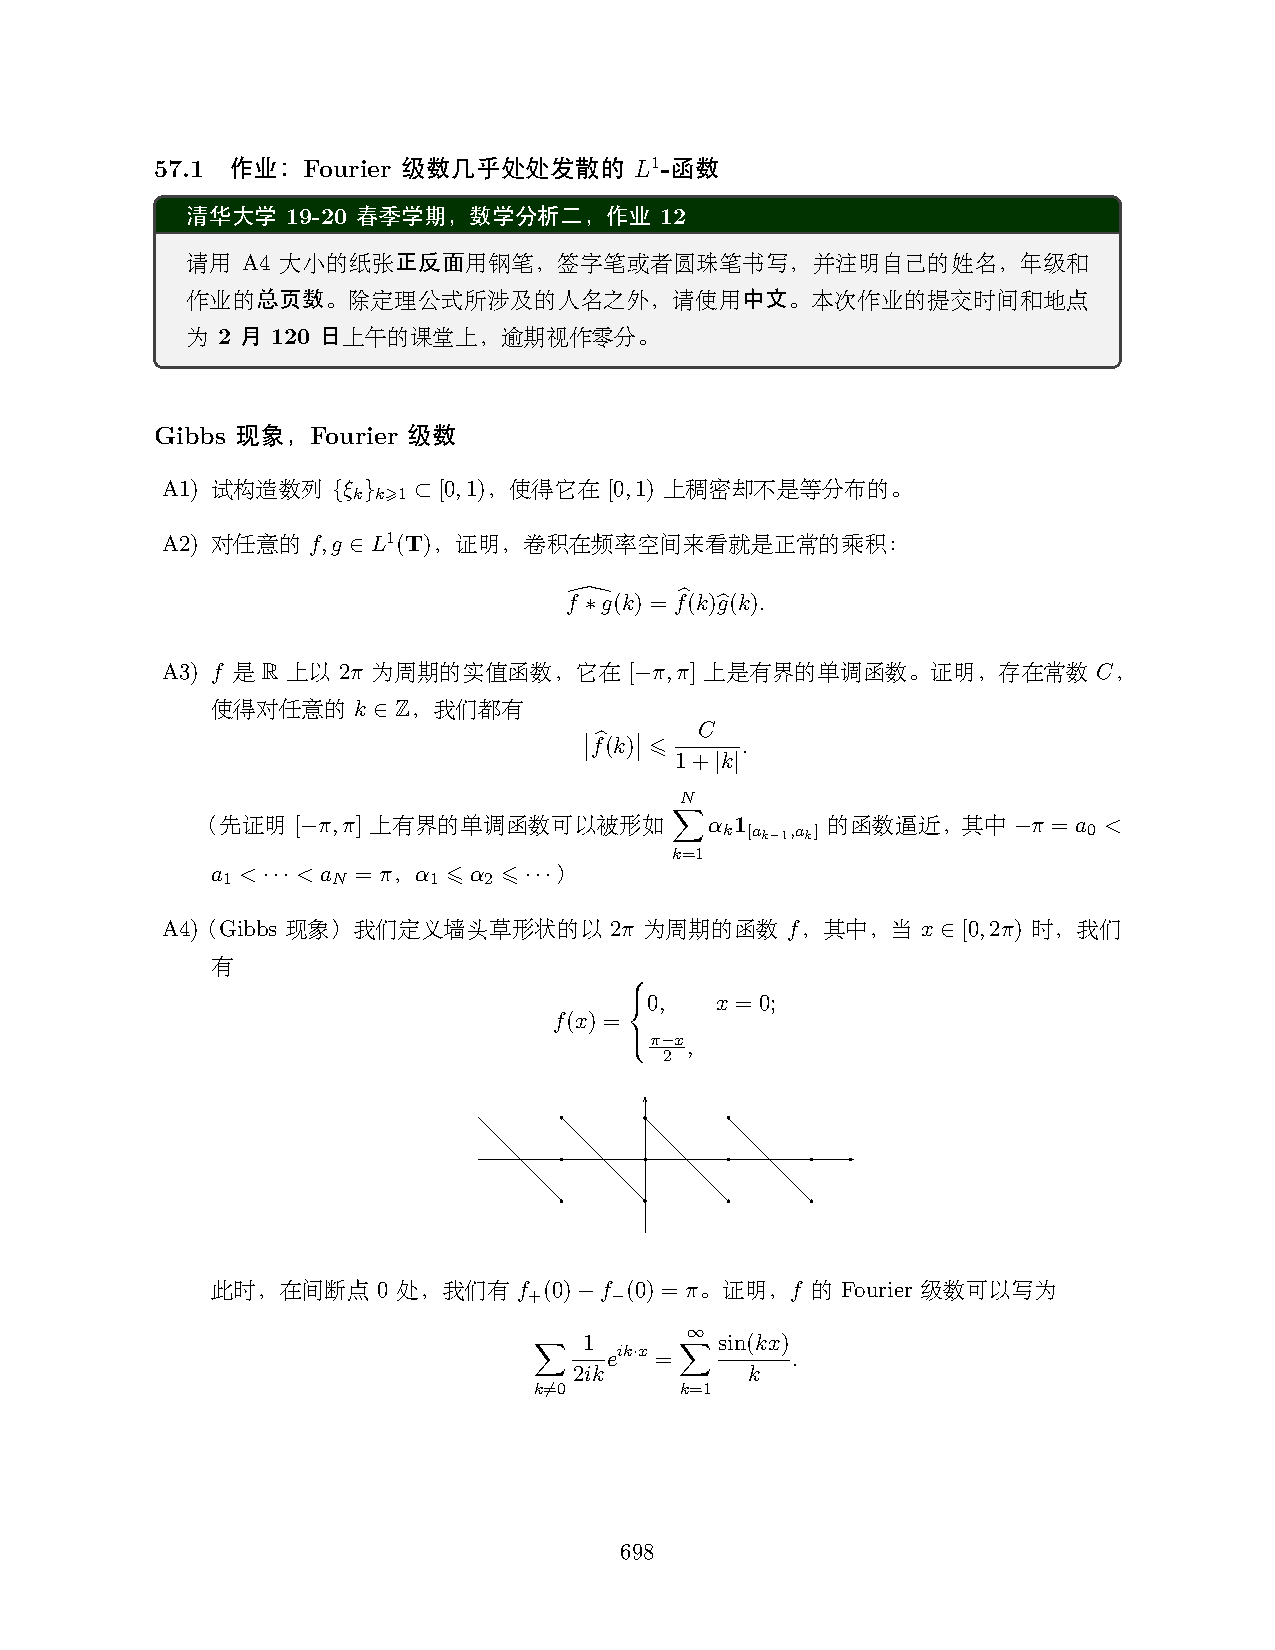
\includepdf[pages=-,pagecommand={\thispagestyle{empty}},scale=.94]{original.pdf}}

\begin{document}
\sourceintro{57.1 作业：Gibbs现象与几乎处处发散的Fourier级数}{57.1}{698--703}
\section*{所用知识}
第43--57讲的卷积、Fubini、$L^2$ Fourier理论、Dirichlet核与有界变差收敛。Kolmogorov反例按题目逐步构造；末题不调用Carleson定理，而直接利用所构造函数的正尖峰证明不属于$L^2$。Fourier及卷积均以$\dd x/(2\pi)$归一化，普通测度$m$仍为长度。
\section{Gibbs现象与Fourier性质}
\problem{A1}{构造$[0,1)$中稠密但不等分布的数列。}
列举$\Q\cap[0,1)$为$r_j$，令$\xi_{2^j}=r_j$，其余项为零。数列值域稠密；前$N$项中非零位置至多$\log_2N$个，故落在$[0,1/2)$中的比例趋于$1$，而该区间长度为$1/2$，所以不等分布。
\problem{A2}{对$f,g\in L^1(\T)$证明$\widehat{f*g}(k)=\widehat f(k)\widehat g(k)$。}
双重积分绝对值不超过$\norm f_1\norm g_1$（使用归一化测度），Fubini允许换序，换元$x=y+z$后指数分解成$e^{-iky}e^{-ikz}$，积分乘开即得。
\problem{A3}{周期函数$f$在一周期上有界单调，证明$|\widehat f(k)|\le C/(1+|k|)$。}
设周期内单调变差为$V$，周期接缝另有大小至多$V$的跳跃。对$0<h<2\pi$，在不穿接缝的部分用单调性将$\int|f(x+h)-f(x)|$化为两个端段积分，接缝部分也由$Vh$控制，合计不超过$2Vh$。取$h=\pi/|k|$，平移的Fourier系数乘$e^{ikh}=-1$，故$2|\widehat f(k)|\le(2\pi)^{-1}2Vh=V/|k|$。$k=0$由有界性处理。严格按闭区间两端同值且全闭区间单调会迫使常数；通常此题指一周期半开区间上的单调代表。
\problem{A4（Gibbs）}{令$f(0)=0$，$f(x)=(\pi-x)/2$在$0<x<2\pi$，周期延拓。(1)证明其Fourier级数为$\sum_{k\ne0}e^{ikx}/(2ik)=\sum_{k\ge1}\sin(kx)/k$；(2)核对原文关于$\max_{0<x\le\pi/N}S_Nf(x)-\pi/2$的公式，并证明超调。}
分部积分给出$\widehat f(0)=0$、$\widehat f(k)=1/(2ik)$。令$H=N+1/2$，由$\sum_{k=1}^N\cos(kt)=(D_N(t)-1)/2$积分，得
\[S_Nf(x)=\frac12\int_0^x\frac{\sin(Ht)}{\sin(t/2)}\dd t-\frac x2.\]
对$u=Hx$，在$0\le u\le\pi H/N$上一致有
\[S_Nf(u/H)=\int_0^u\frac{\sin v}{2H\sin(v/(2H))}\dd v-\frac u{2H}\longrightarrow\int_0^u\frac{\sin v}{v}\dd v.\]
右端在$[0,\pi]$递增，故
\[\lim_{N\to\infty}\left(\max_{0<x\le\pi/N}S_Nf(x)-\frac\pi2\right)=\int_0^\pi\frac{\sin v}{v}\dd v-\frac\pi2>0.\]
\fix{原文省略了最外层$\lim_{N\to\infty}$，有限$N$时等式不成立，$N=1$即可反驳。}
正性可由$\int_0^\infty\sin v/v\dd v=\pi/2$与尾部交错波瓣得到：从$\pi$起第一瓣为负，后续绝对值严格递减，故尾积分负。该Dirichlet积分也可由43.1 B6的$\int(1-\cos v)/v^2=\pi/2$经分部积分得出。超调占跳跃$\pi$的比例约$0.08949$。
\problem{A5}{若$f\in C(\T)$，证明$\sum_k\widehat f(k)/k$绝对收敛。}
\fix{必须删去$k=0$项，否则式子无定义。}
连续函数属于$L^2$，由Bessel不等式及Cauchy--Schwarz，
\[\sum_{k\ne0}\frac{|\widehat f(k)|}{|k|}\le\left(\sum_k|\widehat f(k)|^2\right)^{1/2}\left(\sum_{k\ne0}k^{-2}\right)^{1/2}<\infty.\]
\problem{A6}{证明$S(x)=\sum_{n\ge1}\sin^3(nx)/n!$为光滑周期函数，并用$A=\sum\sin(nx)/n!$、$B=\sum\cos(nx)/n!$证明$S=\frac34e^{\cos x}\sin(\sin x)-\frac14e^{\cos3x}\sin(\sin3x)$。}
任意$r$阶导数的级数由$C_r\sum n^r/n!$一致控制，因此逐阶求导成立。由指数幂级数$B+iA=e^{e^{ix}}-1$得$A=e^{\cos x}\sin(\sin x)$。使用$\sin^3t=(3\sin t-\sin3t)/4$便得公式。保留本题的逐阶一致收敛证明。
\section{含参数积分}
令
\[F(t)=\int_0^\infty\frac{1+tx^5+t^2x^{11}}{1+t^4+x^{13}}\dd x,\qquad a_t(x)=\frac{1+tx^5+t^2x^{11}}{1+t^4+x^{12}}.\]
\problem{B1}{证明对每个$t\in\R$，上述$F(t)$良好定义。}
在任意有界$t$区间$|t|\le T$，被积函数的绝对值被
\[C_T\frac{1+x^5+x^{11}}{1+x^{13}}\]
控制，右端在$(0,\infty)$可积（无穷远为$O(x^{-2})$）。故为绝对收敛的Lebesgue积分。
\problem{B2}{证明$F$在$\R$上连续。}
对任意$t_0$在其紧邻域使用B1的统一控制函数，参数逐点连续，由控制收敛定理得到结论。
\problem{B3}{证明$F$可导。}
分母记为$D=1+t^4+x^{13}$，分子为$N=1+tx^5+t^2x^{11}$。则
\[\partial_t(N/D)=\frac{x^5+2tx^{11}}D-\frac{4t^3N}{D^2}.\]
在$|t|\le T$上仍被$C_T(1+x^5+x^{11})/(1+x^{13})$控制。积分求导定理说明$F' =\int\partial_t(N/D)$，并且同一控制还说明$F'\in C(\R)$。
\problem{B4}{计算$\lim_{t\to+\infty}F(t)$。}
令$A=1+t^4$、$c_j=\int_0^\infty u^j/(1+u^{13})\dd u$，$j=0,5,11$。这些数有限且严格正。换元$x=A^{1/13}u$得到
\[F(t)=c_0A^{-12/13}+tc_5A^{-7/13}+t^2c_{11}A^{-1/13}.\]
前两项分别趋于零，最后一项渐近于$c_{11}t^{22/13}$，故极限为$+\infty$。无需计算$c_j$的闭式。
\problem{B5}{证明当$t\ne0$时$\int_0^\infty a_t(x)\dd x$发散。}
$\lim_{x\to\infty}xa_t(x)=t^2>0$，所以从某处起$a_t(x)\ge t^2/(2x)$，积分发散到$+\infty$。
\problem{B6}{证明每个$t\in\R$的反常积分$G(t)=\lim_{T\to\infty}\int_0^Ta_t(x)e^{ix}\dd x$存在。}
$a_t(x)\to0$，且$a_t'(x)=O_t(x^{-2})$，故分部积分得
\[G(t)=-\frac{a_t(0)}i-\frac1i\int_0^\infty a_t'(x)e^{ix}\dd x.\]
右端积分绝对收敛，左端的截断边界项趋于零，从而反常积分存在。
\problem{B7}{证明$G$在$\R$上连续。}
在$|t|\le T$上，$a_t'$在$[0,1]$上一致有界，在$[1,\infty)$上被$C_Tx^{-2}$控制。对B6的绝对收敛表示使用控制收敛，即得连续性。
\problem{B8}{计算$\lim_{t\to+\infty}G(t)$。}
仅把参数极限移入原反常积分不足以证明结论。令$A=1+t^4$，$h_j(u)=u^j/(1+u^{12})$，$j=0,5,11$，则
\[a_t(x)=A^{-1}h_0(x/A^{1/12})+tA^{-7/12}h_5(x/A^{1/12})+t^2A^{-1/12}h_{11}(x/A^{1/12}).\]
各$h_j^{(8)}\in L^1(0,\infty)$，这是因为它们在零点光滑、在无穷远分别为$O(u^{j-20})$。所以
\[\norm{a_t^{(8)}}_1\le C\{A^{-19/12}+tA^{-14/12}+t^2A^{-8/12}\}\longrightarrow0.\]
连续分部积分八次的边界项只涉及$a_t^{(r)}(0)$，$0\le r\le7$。其非零项仅$r=0,5$，分别为$1/A$和$5!t/A$，均趋零；无穷远的各阶导数均趋零。因此$|G(t)|\le A^{-1}+5!t/A+\norm{a_t^{(8)}}_1\to0$。
\section{Laplace变换}
以下$f,g\in L^1(0,\infty)$，定义$Lf(x)=\int_0^\infty f(t)e^{-xt}\dd t$，$x>0$。
\problem{C1}{证明$Lf\in C^\infty(0,\infty)$。}
对紧区间$x\in[a,b]\subset(0,\infty)$和任意整数$r\ge0$，$t^re^{-xt}|f(t)|\le C_{r,a}|f(t)|$。反复使用控制收敛与积分求导定理即可。
\problem{C2}{证明$(Lf)^{(r)}(x)=\int_0^\infty(-t)^rf(t)e^{-xt}\dd t$。}
C1的每一次求导均可移入积分，归纳即得；该公式也说明各阶导数连续。
\problem{C3}{令$(f\bullet g)(t)=\int_0^tf(\tau)g(t-\tau)\dd\tau$，证明$f\bullet g=g\bullet f$。}
\fix{一般$L^1$函数的卷积应按几乎处处定义来理解；Tonelli给出$\norm{f\bullet g}_1\le\norm f_1\norm g_1$。在绝对收敛的$t$处换元$\sigma=t-\tau$得到交换律，因而作为$L^1$元素相等。}
\problem{C4}{证明$L(f\bullet g)(x)=(Lf)(x)(Lg)(x)$。}
双重积分绝对值至多$\norm f_1\norm g_1$，所以可用Fubini。以$t=\tau+\sigma$将三角形区域化成第一象限，得到
\[\int_0^\infty\int_0^t f(\tau)g(t-\tau)e^{-xt}\dd\tau\dd t=\int_0^\infty\int_0^\infty f(\tau)g(\sigma)e^{-x\tau}e^{-x\sigma}\dd\sigma\dd\tau.\]

\section{Kolmogorov反例：有限尖峰构造}
固定整数$n\ge10000$。令$m_1=n$，对$k\ge2$选足够大的奇数$\lambda_k$使$2m_k+1=\lambda_k(2n+1)$；等价地$\lambda_1=1$。令
\[A_k=\frac{4k\pi}{2n+1},\quad\Delta_k=[A_k-m_k^{-2},A_k+m_k^{-2}],\quad\varphi_n=\sum_{k=1}^n\frac{m_k^2}{n}\ind_{\Delta_k},\]
\[\sigma_k=[A_{k-1}+2n^{-2},A_k-2n^{-2}],\quad 2\le k\le n,\qquad D_m(t)=\sum_{|j|\le m}e^{ijt}=\frac{\sin((m+1/2)t)}{\sin(t/2)}.\]
定义$I_{k,s}(x)=\frac{m_s^2}{2\pi n}\int_{\Delta_s}D_{m_k}(x-t)\dd t$。这就是原文的$I_{m_k,\Delta_s}$。
\problem{K1}{证明$\int_0^{2\pi}\varphi_n=2$，且$S_{m_k}\varphi_n=\sum_{s=1}^nI_{k,s}$。}
每个尖峰高$m_s^2/n$、宽$2m_s^{-2}$，积分$2/n$，总和为$2$。Dirichlet核部分和卷积公式和有限线性性给出第二式。各$\Delta_s$均在$(0,2\pi)$内。
\problem{K2**}{证明$\sup_{N\ge0,x\in[0,2\pi]}|S_N\varphi_n(x)|<\infty$。}
先证明$H_N(t)=\sum_{j=1}^N\sin(jt)/j$对$N,t$一致有界。利用对称与周期可设$0<t\le\pi$；前$j\le1/t$的和绝对值$\le\sum t\le1$。后段分部求和，$|\sum_{j=p}^q e^{ijt}|\le2/|1-e^{it}|\le C/t$，再用$1/j$单调递减，得尾和$\le C/(tp)\le C'$；当$1/t<1$时全段用相同估计。于是$H_N$一致有界。单个区间$[a,b]$的部分和是$(b-a)/(2\pi)+[H_N(x-a)-H_N(x-b)]/\pi$，故一致有界；$\varphi_n$为有限个此类函数的线性组合，所求上界有限，可依赖$n,m_s$。
\problem{K3*}{证明可递归选择奇数$\lambda_k$使$\sigma_k,\Delta_s$两两不交，并对$k\ge2,x\in\sigma_k$有$|\sum_{s<k}I_{k,s}(x)|\le1$。}
中心间距$4\pi/(2n+1)>2/n^2$，而各半宽$\le n^{-2}$，给出不交性（端点间保留严格间隙）。固定之前的$m_s$，$x\in\sigma_k$到$\Delta_s$及模$2\pi$奇点均有正的统一距离。把$I_{k,s}$写成振荡正弦乘$1/\sin((x-t)/2)$的积分，对$t$分部积分，其绝对值$\le C_{n,s}/(m_k+1/2)$，常数在$\sigma_k$上一致。奇数$\lambda_k$可任意大，故可令有限个先前项的总和$\le1$；同时可附加后文K9所需的更大下界。原文$m_1=n$与任意$\lambda_1$并不独立，必须取$\lambda_1=1$。
\problem{K4}{证明$|D_{m_k}'(x)|\le2m_k^2$。}
对有限指数和求导，$|D_m'|\le\sum_{j=-m}^m|j|=m(m+1)\le2m^2$。
\problem{K5}{当$s\ge k,x\in\sigma_k$时证明
\[I_{k,s}=\frac{\sin((m_k+1/2)(x-A_s))}{n\pi\sin((x-A_s)/2)}+R_{k,s},\quad |R_{k,s}|\le4/n,\]
其中$R_{k,s}=\frac{m_s^2}{2\pi n}\int_{\Delta_s}[D_{m_k}(x-t)-D_{m_k}(x-A_s)]\dd t$。}
以中心值代替被积核，常数项的积分因宽度为$2m_s^{-2}$正好给出主项。由K4及$|t-A_s|\le m_s^{-2}$，差至多$2m_k^2m_s^{-2}$，故余项$\le2m_k^2/(\pi n m_s^2)\le2/(\pi n)<4/n$。
\problem{K6}{证明对$x\in\sigma_k$，
\[\abs{\sum_{s=k}^nI_{k,s}}\ge\frac{|\sin((m_k+1/2)(x-A_k))|}{n\pi}\abs{\sum_{s=k}^n\frac1{\sin((x-A_s)/2)}}-4.\]}
因$(m_k+1/2)A_s=2\pi\lambda_ks$，所有分子正弦相等。K5的主项可提取共同分子，余项总绝对值至多$4$，由反三角不等式得结论。
\problem{K7}{证明$x\in\sigma_k$时$\frac1n|\sum_{s=k}^n1/\sin((x-A_s)/2)|\ge\pi^{-1}\sum_{\ell=1}^{n-k}1/\ell$。}
所有$A_s-x$在$(0,2\pi)$内，分母全负，所以取绝对值后无抵消。又$\sin((A_s-x)/2)\le(A_s-x)/2\le2\pi(s-k+1)/(2n+1)$，所以每项的绝对值至少$(2n+1)/(2\pi(s-k+1))$。求和、除以$n$，再舍去最后一个正项即得。
\problem{K8}{若$2\le k\le n-\sqrt n$，证明$|\sum_{s=k}^nI_{k,s}(x)|\ge |\sin((m_k+1/2)(x-A_k))|\log n/(2\pi^2)-8$。}
K7中的调和和至少$\log(n-k+1)\ge\frac12\log n$。代入K6得到更强的常数$-4$，因而原式成立。
\problem{K9}{若$m_2$充分大，证明在$[A_{k-1},A_k]$内满足$|\sin((m_k+1/2)(x-A_k))|<2\pi^2/\sqrt{\log n}$的集合测度为$O(1/(n\sqrt{\log n}))$。}
记阈值$\delta$。当$0<\delta<1/2$时，一周期内$|\sin|<\delta$的比例至多$C\delta$，端点不足一周期产生$C/(m_k+1/2)$的误差。因此坏集长度$\le C\delta/n+C/m_k$。递归选$m_2\ge n\sqrt{\log n}$并增大固定常数，后续$m_k\ge m_2$，即可得到所需界。有限个阈值不小的$n$可放入统一常数，不影响渐近结论。
\problem{K10}{令$E_{n,k}=\{x\in\sigma_k:|\sin((m_k+1/2)(x-A_k))|\ge2\pi^2/\sqrt{\log n}\}$，$E_n=\bigcup_{2\le k\le n-\sqrt n}E_{n,k}$。证明$m(E_n)\to2\pi$。}
被丢弃的首尾$O(\sqrt n)$个中心间隔总长$O(n^{-1/2})$；每个$\sigma_k$端部缩短$4/n^2$，总损失$O(1/n)$；K9的坏集总损失$O((\log n)^{-1/2})$。三项均趋零，且$E_n\subset[0,2\pi]$。
\problem{K11}{证明$x\in E_{n,k}$时$|S_{m_k}\varphi_n(x)|\ge\sqrt{\log n}-9$。}
K8与阈值给出尾项和$\ge\sqrt{\log n}-8$；K3的先前项总绝对值$\le1$，再次用反三角不等式。
\section{抽子列与无穷叠加}
\problem{K12}{证明存在非负周期函数列$\varphi_n$、集合$E_n$、整数$q_n$与递增正数$M_n\to\infty$，使$\int\varphi_n=2$、每个$\sup_{N,x}|S_N\varphi_n|<\infty$，$m(E_n)\to2\pi$，且每个$x\in E_n$存在$N_x\le q_n$使$|S_{N_x}\varphi_n(x)|\ge M_n$。}
为避免$\sqrt{\log n}-9$在前面若干项非正，另取严格递增构造参数$\nu_n$，使$\nu_n\ge n^2$、$\sqrt{\log\nu_n}-9\ge n$。把原构造的$\varphi_{\nu_n},E_{\nu_n}$重新编号为$\varphi_n,E_n$，令$M_n=n$、$q_n=m_{\nu_n}$（该构造的最大频率）。K1、K2、K10、K11给出所有要求。
\fix{原文将$E_n$称为“子区间序列”，实际构造给出可测子集，且每个是有限个区间的并，并非单个区间。}
\problem{K13}{证明可再选函数列$\phi_n$、集合$E_n$和$q_n,M_n$使：(a)$M_1\ge2$且$M_n\ge2M_{n-1}$；(b)$\int\phi_n=2$且$\sum_{k<n}\sup_{N,x}|S_N\phi_k|<\sqrt{M_n}/2$；(c)$\max_{k<n}q_k\le\sqrt{M_n}/2^n$；(d)$m(E_n)\to2\pi$且在$E_n$上有某个$N_x\le q_n$使$|S_{N_x}\phi_n|\ge M_n$。}
递归从K12抽取子列。先前函数的有限个上界、频率及$M_{n-1}$都已固定，K12的$M_j=j\to\infty$允许选择下一指标足够大，使(a)--(c)同时成立。保留对应的$E_j,q_j$，则(d)仍成立。函数非负及质量不变。记所抽K12指标为$j_n$，则$M_n=j_n$且其底层参数$\nu_{j_n}\ge j_n^2$，留待K20使用。
\problem{K14}{令$f=\sum_{n\ge1}\phi_n/\sqrt{M_n}$，证明它在$L^1$中良定义且级数几乎处处收敛。}
由(a)，$M_n\ge2^n$。因此$\sum_n\norm{\phi_n/\sqrt{M_n}}_1=2\sum_nM_n^{-1/2}<\infty$。非负函数单调收敛给出有限积分，因而和几乎处处有限；尾范数趋零又给出$L^1$收敛。
\problem{K15}{证明$S_Nf=S_N(\phi_n/\sqrt{M_n})+\sum_{s<n}S_N(\phi_s/\sqrt{M_s})+\sum_{s>n}S_N(\phi_s/\sqrt{M_s})$。}
对固定$N$，$D_N$有界，$L^1$收敛可移入卷积；且所得级数对$x$一致绝对收敛，因为$\norm{S_Nh}_\infty\le(2N+1)\norm h_{L^1(\dd x)}/(2\pi)$。故可合法分成三段。
\problem{K16}{原文声称对$x\in E_n$存在$N_x\le\sqrt{M_n}/2^n$使$|S_{N_x}(\phi_n/\sqrt{M_n})(x)|\ge\sqrt{M_n}$。}
\fix{这一频率上界不由K13推出，应为$N_x\le q_n$。K13(c)控制的是\emph{先前}的$q_k$，不能用于同一$n$。按修正上界，结论立即由K13(d)除以$\sqrt{M_n}$得到。后面的尾项估计只需这个正确上界。}
\problem{K17}{证明对任意$N$，$|\sum_{s<n}S_N(\phi_s/\sqrt{M_s})(x)|\le\sqrt{M_n}/2$。}
因为$\sqrt{M_s}\ge1$，左边至多$\sum_{s<n}\sup_{N,x}|S_N\phi_s|$，由K13(b)得到。
\problem{K18}{证明尾项$|\sum_{s>n}S_N(\phi_s/\sqrt{M_s})(x)|\le100/2^n$，并说明频率范围。}
\fix{该估计需要$N\le q_n$。原文未写范围，若对任意$N$断言则没有这些条件的支持；证明中只在K16选择的$N_x\le q_n$处使用。}
对$s>n$，K13(c)使$q_n/\sqrt{M_s}\le2^{-s}$。由$\int\phi_s=2$及$|D_N|\le2N+1$，
\[\abs{\sum_{s>n}S_N\frac{\phi_s}{\sqrt{M_s}}}\le\frac{2q_n+1}{\pi}\sum_{s>n}\frac1{\sqrt{M_s}}\le\frac3\pi\sum_{s>n}2^{-s}<100\,2^{-n},\]
其中$q_n\ge1$。这同时说明常数$100$远非必要。
\problem{K19}{证明$f$的Fourier部分和几乎处处发散。}
由K15--K18，对$x\in E_n$有某个$N_x\le q_n$满足$|S_{N_x}f(x)|\ge\sqrt{M_n}/2-100\,2^{-n}\to\infty$。又$m(E_n)\to2\pi$蕴含$m(\limsup E_n)=2\pi$：每个尾部并集的测度至少$\sup_{n\ge r}m(E_n)=2\pi$。所以几乎每个$x$在无穷多个$E_n$中，部分和绝对值无界；这些频率必趋于无穷的某个子列，因为有限个固定部分和均为有限数。故几乎处处发散，实际上$\limsup_N|S_Nf|=\infty$。
\problem{K20}{证明$f\notin L^2([0,2\pi])$。}
不用Carleson定理。原有限构造参数为$\nu$时，各尖峰不交且$m_s\ge\nu$，所以
\[\norm{\varphi_\nu}_2^2=\frac2{\nu^2}\sum_{s=1}^{\nu}m_s^2\ge2\nu.\]
在K13抽取的第$n$项，底层参数$\nu_{j_n}\ge j_n^2=M_n^2$。由于$f\ge\phi_n/\sqrt{M_n}\ge0$，
\[\int f^2\ge\frac{\norm{\phi_n}_2^2}{M_n}\ge\frac{2\nu_{j_n}}{M_n}\ge2M_n\to\infty.\]
所以$f$不可平方积。这也直接说明为什么该反例不会与$L^2$理论冲突。
\originalpages
\end{document}
